\PassOptionsToPackage{unicode=true}{hyperref} % options for packages loaded elsewhere
\PassOptionsToPackage{hyphens}{url}
%
\documentclass[]{article}
\usepackage{lmodern}
\usepackage{amssymb,amsmath}
\usepackage{ifxetex,ifluatex}
\usepackage{fixltx2e} % provides \textsubscript
\ifnum 0\ifxetex 1\fi\ifluatex 1\fi=0 % if pdftex
  \usepackage[T1]{fontenc}
  \usepackage[utf8]{inputenc}
  \usepackage{textcomp} % provides euro and other symbols
\else % if luatex or xelatex
  \usepackage{unicode-math}
  \defaultfontfeatures{Ligatures=TeX,Scale=MatchLowercase}
\fi
% use upquote if available, for straight quotes in verbatim environments
\IfFileExists{upquote.sty}{\usepackage{upquote}}{}
% use microtype if available
\IfFileExists{microtype.sty}{%
\usepackage[]{microtype}
\UseMicrotypeSet[protrusion]{basicmath} % disable protrusion for tt fonts
}{}
\IfFileExists{parskip.sty}{%
\usepackage{parskip}
}{% else
\setlength{\parindent}{0pt}
\setlength{\parskip}{6pt plus 2pt minus 1pt}
}
\usepackage{hyperref}
\hypersetup{
            pdftitle={Lab 1 - Graphical Models},
            pdfauthor={Alice Velander},
            pdfborder={0 0 0},
            breaklinks=true}
\urlstyle{same}  % don't use monospace font for urls
\usepackage[margin=1in]{geometry}
\usepackage{color}
\usepackage{fancyvrb}
\newcommand{\VerbBar}{|}
\newcommand{\VERB}{\Verb[commandchars=\\\{\}]}
\DefineVerbatimEnvironment{Highlighting}{Verbatim}{commandchars=\\\{\}}
% Add ',fontsize=\small' for more characters per line
\usepackage{framed}
\definecolor{shadecolor}{RGB}{248,248,248}
\newenvironment{Shaded}{\begin{snugshade}}{\end{snugshade}}
\newcommand{\AlertTok}[1]{\textcolor[rgb]{0.94,0.16,0.16}{#1}}
\newcommand{\AnnotationTok}[1]{\textcolor[rgb]{0.56,0.35,0.01}{\textbf{\textit{#1}}}}
\newcommand{\AttributeTok}[1]{\textcolor[rgb]{0.77,0.63,0.00}{#1}}
\newcommand{\BaseNTok}[1]{\textcolor[rgb]{0.00,0.00,0.81}{#1}}
\newcommand{\BuiltInTok}[1]{#1}
\newcommand{\CharTok}[1]{\textcolor[rgb]{0.31,0.60,0.02}{#1}}
\newcommand{\CommentTok}[1]{\textcolor[rgb]{0.56,0.35,0.01}{\textit{#1}}}
\newcommand{\CommentVarTok}[1]{\textcolor[rgb]{0.56,0.35,0.01}{\textbf{\textit{#1}}}}
\newcommand{\ConstantTok}[1]{\textcolor[rgb]{0.00,0.00,0.00}{#1}}
\newcommand{\ControlFlowTok}[1]{\textcolor[rgb]{0.13,0.29,0.53}{\textbf{#1}}}
\newcommand{\DataTypeTok}[1]{\textcolor[rgb]{0.13,0.29,0.53}{#1}}
\newcommand{\DecValTok}[1]{\textcolor[rgb]{0.00,0.00,0.81}{#1}}
\newcommand{\DocumentationTok}[1]{\textcolor[rgb]{0.56,0.35,0.01}{\textbf{\textit{#1}}}}
\newcommand{\ErrorTok}[1]{\textcolor[rgb]{0.64,0.00,0.00}{\textbf{#1}}}
\newcommand{\ExtensionTok}[1]{#1}
\newcommand{\FloatTok}[1]{\textcolor[rgb]{0.00,0.00,0.81}{#1}}
\newcommand{\FunctionTok}[1]{\textcolor[rgb]{0.00,0.00,0.00}{#1}}
\newcommand{\ImportTok}[1]{#1}
\newcommand{\InformationTok}[1]{\textcolor[rgb]{0.56,0.35,0.01}{\textbf{\textit{#1}}}}
\newcommand{\KeywordTok}[1]{\textcolor[rgb]{0.13,0.29,0.53}{\textbf{#1}}}
\newcommand{\NormalTok}[1]{#1}
\newcommand{\OperatorTok}[1]{\textcolor[rgb]{0.81,0.36,0.00}{\textbf{#1}}}
\newcommand{\OtherTok}[1]{\textcolor[rgb]{0.56,0.35,0.01}{#1}}
\newcommand{\PreprocessorTok}[1]{\textcolor[rgb]{0.56,0.35,0.01}{\textit{#1}}}
\newcommand{\RegionMarkerTok}[1]{#1}
\newcommand{\SpecialCharTok}[1]{\textcolor[rgb]{0.00,0.00,0.00}{#1}}
\newcommand{\SpecialStringTok}[1]{\textcolor[rgb]{0.31,0.60,0.02}{#1}}
\newcommand{\StringTok}[1]{\textcolor[rgb]{0.31,0.60,0.02}{#1}}
\newcommand{\VariableTok}[1]{\textcolor[rgb]{0.00,0.00,0.00}{#1}}
\newcommand{\VerbatimStringTok}[1]{\textcolor[rgb]{0.31,0.60,0.02}{#1}}
\newcommand{\WarningTok}[1]{\textcolor[rgb]{0.56,0.35,0.01}{\textbf{\textit{#1}}}}
\usepackage{graphicx,grffile}
\makeatletter
\def\maxwidth{\ifdim\Gin@nat@width>\linewidth\linewidth\else\Gin@nat@width\fi}
\def\maxheight{\ifdim\Gin@nat@height>\textheight\textheight\else\Gin@nat@height\fi}
\makeatother
% Scale images if necessary, so that they will not overflow the page
% margins by default, and it is still possible to overwrite the defaults
% using explicit options in \includegraphics[width, height, ...]{}
\setkeys{Gin}{width=\maxwidth,height=\maxheight,keepaspectratio}
\setlength{\emergencystretch}{3em}  % prevent overfull lines
\providecommand{\tightlist}{%
  \setlength{\itemsep}{0pt}\setlength{\parskip}{0pt}}
\setcounter{secnumdepth}{0}
% Redefines (sub)paragraphs to behave more like sections
\ifx\paragraph\undefined\else
\let\oldparagraph\paragraph
\renewcommand{\paragraph}[1]{\oldparagraph{#1}\mbox{}}
\fi
\ifx\subparagraph\undefined\else
\let\oldsubparagraph\subparagraph
\renewcommand{\subparagraph}[1]{\oldsubparagraph{#1}\mbox{}}
\fi

% set default figure placement to htbp
\makeatletter
\def\fps@figure{htbp}
\makeatother

\renewcommand{\linethickness}{0.05em}

\title{Lab 1 - Graphical Models}
\author{Alice Velander}
\date{13/9/2020}

\begin{document}
\maketitle

\begin{Shaded}
\begin{Highlighting}[]
\NormalTok{knitr}\OperatorTok{::}\NormalTok{opts_chunk}\OperatorTok{$}\KeywordTok{set}\NormalTok{(}\DataTypeTok{echo =} \OtherTok{TRUE}\NormalTok{)}
\end{Highlighting}
\end{Shaded}

\hypertarget{task-1---show-that-multiple-runs-of-the-hill-climbing-algorithm-can-return-non-equivalent-bayesian-network-bn-structures.}{%
\subsection{Task 1 - Show that multiple runs of the hill-climbing
algorithm can return non-equivalent Bayesian network (BN)
structures.}\label{task-1---show-that-multiple-runs-of-the-hill-climbing-algorithm-can-return-non-equivalent-bayesian-network-bn-structures.}}

\begin{Shaded}
\begin{Highlighting}[]
\CommentTok{#install.packages("bnlearn")}
\KeywordTok{library}\NormalTok{(bnlearn)}

\KeywordTok{data}\NormalTok{(}\StringTok{"asia"}\NormalTok{)}
\NormalTok{amount=}\DecValTok{5}
\NormalTok{network =}\StringTok{ }\KeywordTok{list}\NormalTok{()}

\CommentTok{#save different networks created by the hillclimbing method in a list}
\ControlFlowTok{for}\NormalTok{ (i }\ControlFlowTok{in} \DecValTok{1}\OperatorTok{:}\NormalTok{amount)\{}
\NormalTok{  climb =}\StringTok{ }\KeywordTok{hc}\NormalTok{(asia, }\DataTypeTok{start=}\OtherTok{NULL}\NormalTok{, }\DataTypeTok{restart =} \DecValTok{10}\NormalTok{, }\DataTypeTok{optimized =} \OtherTok{FALSE}\NormalTok{)}
\NormalTok{  network[[i]] =}\StringTok{ }\NormalTok{climb   }
\NormalTok{\}}

\KeywordTok{par}\NormalTok{(}\DataTypeTok{mfrow=}\KeywordTok{c}\NormalTok{(}\DecValTok{1}\NormalTok{,}\DecValTok{1}\NormalTok{))}
\CommentTok{#compare the networks to each other }
\NormalTok{stop=}\OtherTok{FALSE}
\ControlFlowTok{for}\NormalTok{ (i }\ControlFlowTok{in} \DecValTok{1}\OperatorTok{:}\NormalTok{(amount}\DecValTok{-1}\NormalTok{))\{}
  \ControlFlowTok{for}\NormalTok{ (j }\ControlFlowTok{in}\NormalTok{ (i}\OperatorTok{+}\DecValTok{1}\NormalTok{)}\OperatorTok{:}\NormalTok{(amount))\{}
    \ControlFlowTok{if}\NormalTok{( }\KeywordTok{all.equal}\NormalTok{(network[[i]], network[[j]]) }\OperatorTok{!=}\StringTok{ }\OtherTok{TRUE}\NormalTok{ )\{}
      \KeywordTok{plot}\NormalTok{(network[[j]])}
      \KeywordTok{plot}\NormalTok{(network[[i]])}
\NormalTok{      stop =}\StringTok{ }\OtherTok{TRUE}
      \ControlFlowTok{break}
\NormalTok{    \}}
\NormalTok{  \}}
  \ControlFlowTok{if}\NormalTok{ (stop)\{}\ControlFlowTok{break}\NormalTok{\}}
\NormalTok{\}}
\end{Highlighting}
\end{Shaded}

\begin{center}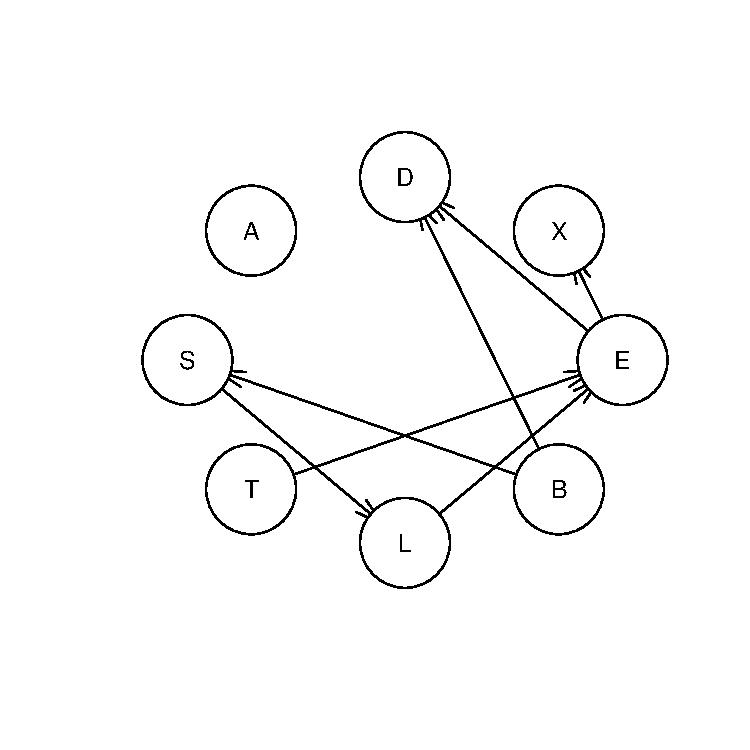
\includegraphics[width=.49\linewidth]{Lab1_graphical_models_alive213_files/figure-latex/unnamed-chunk-3-1} 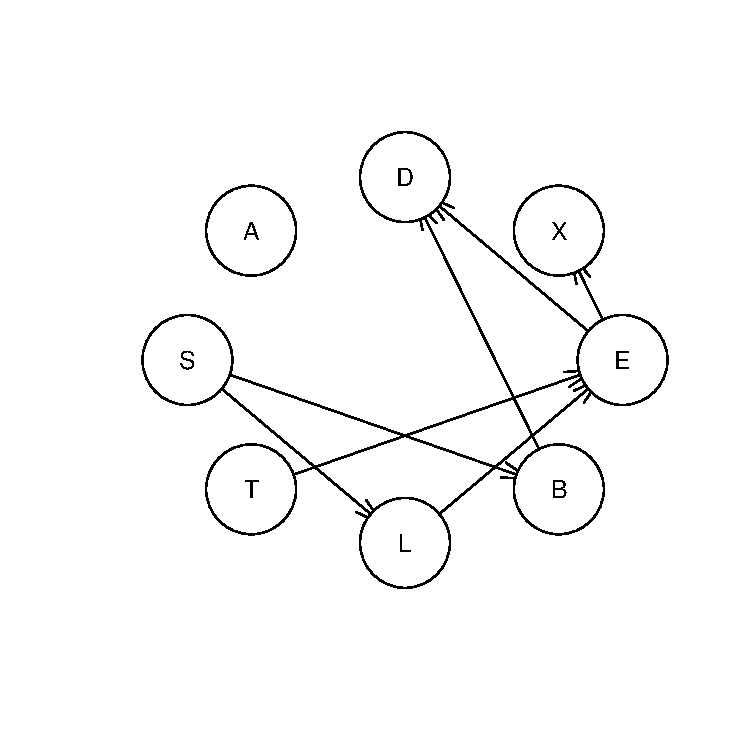
\includegraphics[width=.49\linewidth]{Lab1_graphical_models_alive213_files/figure-latex/unnamed-chunk-3-2} \end{center}

The hill-climbing method starts with an empty DAG and add/remove/reverse
edges given that it increases the total log bayesian score. The reason
why HC results in different DAGs is because somethimes directions of an
edge doesn't give higher or lower score, since it's the same statistical
model. This results in a randomized chosen direction of edge. We get
different local optimum, and results in different networks in different
iterations.

\hypertarget{task-2---use-the-bn-learned-to-classify-the-remaining-20-of-the-asia-dataset-in-two-classes-s-yes-and-s-no.}{%
\subsection{Task 2 - Use the BN learned to classify the remaining 20 \%
of the Asia dataset in two classes: S = yes and S =
no.}\label{task-2---use-the-bn-learned-to-classify-the-remaining-20-of-the-asia-dataset-in-two-classes-s-yes-and-s-no.}}

\begin{Shaded}
\begin{Highlighting}[]
\NormalTok{dag =}\StringTok{ }\KeywordTok{model2network}\NormalTok{(}\StringTok{"[A][S][T|A][L|S][B|S][D|B:E][E|T:L][X|E]"}\NormalTok{)}

\CommentTok{#split dataset into traning and test}
\NormalTok{n=}\KeywordTok{dim}\NormalTok{(asia)[}\DecValTok{1}\NormalTok{] }
\KeywordTok{set.seed}\NormalTok{(}\DecValTok{12345}\NormalTok{) }
\NormalTok{id=}\KeywordTok{sample}\NormalTok{(}\DecValTok{1}\OperatorTok{:}\NormalTok{n, }\KeywordTok{floor}\NormalTok{(n}\OperatorTok{*}\FloatTok{0.8}\NormalTok{)) }

\NormalTok{train=asia[id,]}
\NormalTok{test=asia[}\OperatorTok{-}\NormalTok{id,]}

\CommentTok{#install.packages("gRain")}
\KeywordTok{library}\NormalTok{(gRain)}

\CommentTok{#create network from train}
\NormalTok{network =}\StringTok{ }\KeywordTok{hc}\NormalTok{(train, }\DataTypeTok{start=}\OtherTok{NULL}\NormalTok{, }\DataTypeTok{restart =} \DecValTok{10}\NormalTok{, }\DataTypeTok{optimized =} \OtherTok{FALSE}\NormalTok{)}
\CommentTok{#learn parameters for created network, based on same dataset,}
\CommentTok{#get conditional probabiities in BN - needed for cliques}
\NormalTok{network_parameters =}\StringTok{ }\KeywordTok{bn.fit}\NormalTok{(network, }\DataTypeTok{data =}\NormalTok{ train)}
\CommentTok{#parameters for created network, see dependencies in matrices below}
\CommentTok{#coefficients(network_parameters)}

\CommentTok{#find potentials for cliques, checking all independencies }
\CommentTok{#Moralize, triangulaize - we get MN - Graphical independence network (grain)}
\NormalTok{graphical_Ind_network =}\StringTok{ }\KeywordTok{as.grain}\NormalTok{(network_parameters)}

\CommentTok{#Create junction tree - R, seperators - needed to estimate potential cliques - information on how nodes inference - dependencies }
\NormalTok{junc_tree =}\StringTok{ }\KeywordTok{compile}\NormalTok{(graphical_Ind_network)}
\CommentTok{#We get our final Markov Network:}
\KeywordTok{plot}\NormalTok{(junc_tree)}
\end{Highlighting}
\end{Shaded}

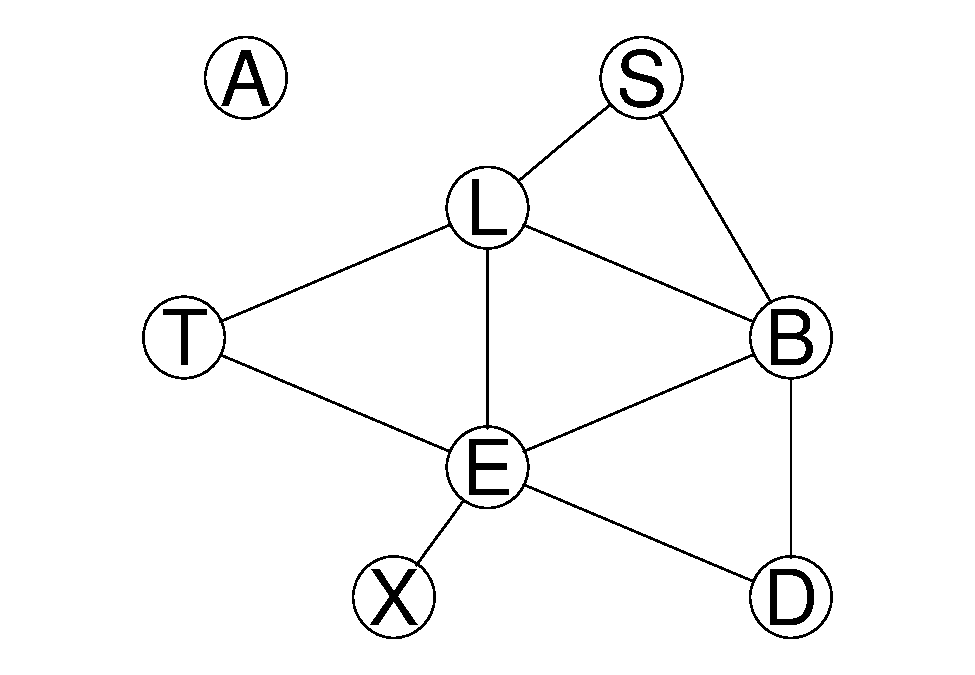
\includegraphics{Lab1_graphical_models_alive213_files/figure-latex/unnamed-chunk-4-1.pdf}

\begin{Shaded}
\begin{Highlighting}[]
\CommentTok{#Classification for testdata!}
\NormalTok{pred_node=}\KeywordTok{c}\NormalTok{(}\StringTok{"S"}\NormalTok{)}
\NormalTok{answer =}\StringTok{ }\NormalTok{test[,}\StringTok{"S"}\NormalTok{]}
\NormalTok{observed =}\StringTok{ }\NormalTok{test[,}\OperatorTok{-}\DecValTok{2}\NormalTok{]}
\NormalTok{nodes =}\StringTok{ }\KeywordTok{c}\NormalTok{(}\StringTok{"A"}\NormalTok{, }\StringTok{"T"}\NormalTok{, }\StringTok{"L"}\NormalTok{, }\StringTok{"B"}\NormalTok{, }\StringTok{"E"}\NormalTok{, }\StringTok{"X"}\NormalTok{, }\StringTok{"D"}\NormalTok{)}

\NormalTok{missclass_rate =}\StringTok{ }\ControlFlowTok{function}\NormalTok{(table)\{}
  \KeywordTok{return}\NormalTok{(}\DecValTok{1}\OperatorTok{-}\KeywordTok{sum}\NormalTok{(}\KeywordTok{diag}\NormalTok{(table))}\OperatorTok{/}\KeywordTok{sum}\NormalTok{(table))}
\NormalTok{\}}

\NormalTok{predict_BN=}\ControlFlowTok{function}\NormalTok{(network, nodes, pred_nodes, answer, observed)\{}
\NormalTok{  classify=}\KeywordTok{c}\NormalTok{()}
\NormalTok{  nrows=}\KeywordTok{nrow}\NormalTok{(observed)}
  \ControlFlowTok{for}\NormalTok{ (i }\ControlFlowTok{in} \DecValTok{1}\OperatorTok{:}\NormalTok{nrows)\{}
    \CommentTok{#Sorry for fulkod}
\NormalTok{    obs =}\StringTok{ }\KeywordTok{as.character}\NormalTok{(observed[i,])}
\NormalTok{    values=}\KeywordTok{c}\NormalTok{()}
    \ControlFlowTok{for}\NormalTok{ (j }\ControlFlowTok{in} \DecValTok{1}\OperatorTok{:}\KeywordTok{length}\NormalTok{(obs))\{}
      \ControlFlowTok{if}\NormalTok{(obs[j]}\OperatorTok{==}\DecValTok{1}\NormalTok{)\{}
\NormalTok{        values=}\KeywordTok{c}\NormalTok{(values, }\StringTok{"no"}\NormalTok{)}
\NormalTok{      \}}\ControlFlowTok{else}\NormalTok{\{}
\NormalTok{        values=}\StringTok{ }\KeywordTok{c}\NormalTok{(values,}\StringTok{"yes"}\NormalTok{)}
\NormalTok{      \}}
\NormalTok{    \}}
    
    \CommentTok{#predict node S}
    \CommentTok{#Given observations - we update clique potentials}
\NormalTok{    evid =}\StringTok{ }\KeywordTok{setEvidence}\NormalTok{(network, }\DataTypeTok{nodes =}\NormalTok{ nodes, }\DataTypeTok{states =}\NormalTok{ values) }
    \CommentTok{#Given new clique potential - we predict a specific node. }
\NormalTok{    pred =}\StringTok{ }\KeywordTok{querygrain}\NormalTok{(evid, }\DataTypeTok{nodes=}\NormalTok{pred_node)}
    
    \ControlFlowTok{if}\NormalTok{(pred}\OperatorTok{$}\NormalTok{S[}\DecValTok{1}\NormalTok{] }\OperatorTok{>}\StringTok{ }\FloatTok{0.5}\NormalTok{)\{ }\CommentTok{#[1] = predict is NO }
\NormalTok{      classify =}\StringTok{ }\KeywordTok{c}\NormalTok{(classify, }\StringTok{"no"}\NormalTok{)}
\NormalTok{    \} }\ControlFlowTok{else}\NormalTok{ \{}
\NormalTok{      classify =}\StringTok{ }\KeywordTok{c}\NormalTok{(classify, }\StringTok{"yes"}\NormalTok{)}
\NormalTok{    \} }
\NormalTok{  \}}
  
  \CommentTok{#Get confusion matrix}
\NormalTok{  conf_matrix=}\KeywordTok{table}\NormalTok{(answer, classify)}
  
  \KeywordTok{return}\NormalTok{(}\DataTypeTok{confusionmatrix=}\NormalTok{conf_matrix)}
\NormalTok{\}}

\KeywordTok{par}\NormalTok{(}\DataTypeTok{mfrow=}\KeywordTok{c}\NormalTok{(}\DecValTok{1}\NormalTok{,}\DecValTok{2}\NormalTok{))}
\KeywordTok{plot}\NormalTok{(network, }\DataTypeTok{main=}\StringTok{"Created network"}\NormalTok{)}
\KeywordTok{plot}\NormalTok{(dag, }\DataTypeTok{main=}\StringTok{"True network"}\NormalTok{)}
\end{Highlighting}
\end{Shaded}

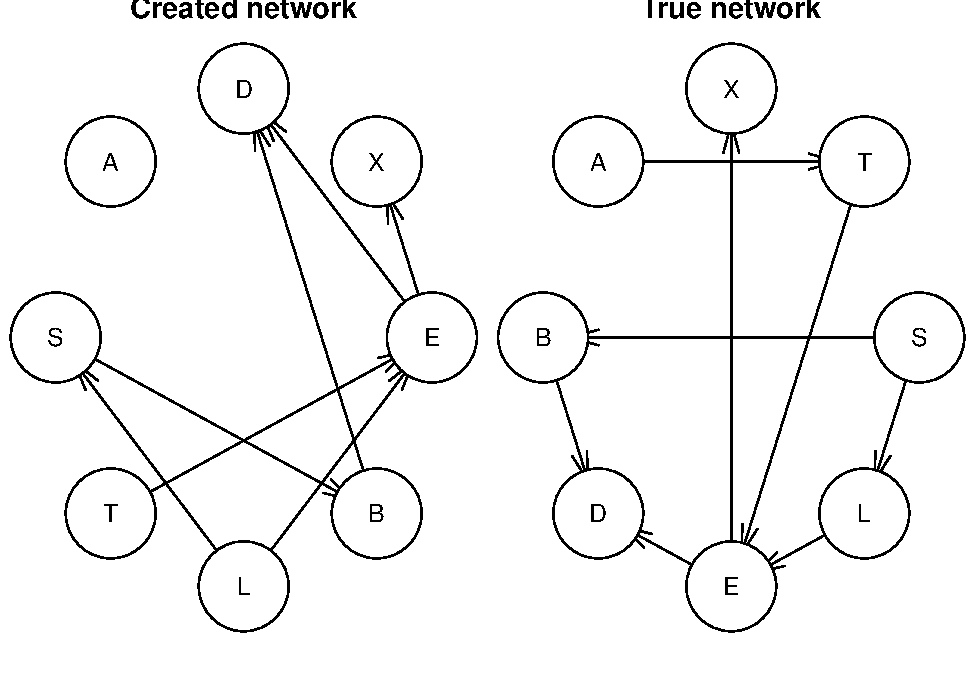
\includegraphics{Lab1_graphical_models_alive213_files/figure-latex/unnamed-chunk-4-2.pdf}

\begin{Shaded}
\begin{Highlighting}[]
\NormalTok{conf_matrix=}\KeywordTok{predict_BN}\NormalTok{(junc_tree,nodes,pred_node, answer, observed)}
\CommentTok{#Confusionmatrix for the created network:}
\KeywordTok{print}\NormalTok{(conf_matrix)}
\end{Highlighting}
\end{Shaded}

\begin{verbatim}
##       classify
## answer  no yes
##    no  337 176
##    yes 121 366
\end{verbatim}

\begin{Shaded}
\begin{Highlighting}[]
\CommentTok{#Misclassificationrate for the created network:}
\KeywordTok{missclass_rate}\NormalTok{(conf_matrix)}
\end{Highlighting}
\end{Shaded}

\begin{verbatim}
## [1] 0.297
\end{verbatim}

\begin{Shaded}
\begin{Highlighting}[]
\CommentTok{#compare results with given dag}
\NormalTok{dag_parameters =}\StringTok{ }\KeywordTok{bn.fit}\NormalTok{(dag, }\DataTypeTok{data =}\NormalTok{ train)}
\NormalTok{graphical_Ind_dag =}\StringTok{ }\KeywordTok{as.grain}\NormalTok{(dag_parameters)}
\NormalTok{dag_tree =}\StringTok{ }\KeywordTok{compile}\NormalTok{(graphical_Ind_dag)}


\NormalTok{conf_matrix_true=}\KeywordTok{predict_BN}\NormalTok{(dag_tree,nodes,pred_node, answer, observed) }\CommentTok{#We get the same results!}

\CommentTok{#Confusionmatrix network for the true network:}
\KeywordTok{print}\NormalTok{(conf_matrix_true)}
\end{Highlighting}
\end{Shaded}

\begin{verbatim}
##       classify
## answer  no yes
##    no  337 176
##    yes 121 366
\end{verbatim}

\begin{Shaded}
\begin{Highlighting}[]
\CommentTok{#Misclassificationrate for the true network:}
\KeywordTok{missclass_rate}\NormalTok{(conf_matrix_true)}
\end{Highlighting}
\end{Shaded}

\begin{verbatim}
## [1] 0.297
\end{verbatim}

We get the same results (confusionmatrix and masclassification rate).
Given the markov network, S is independenten to the remaining nodes in
the network. Comparing the networks, S has the same markov blanket for
both networks. Since the markov blanket is ``the seperators'' from the
rest of the network, it only dependes on those specific nodes. This
gives us the same results, with the two different networks.

\hypertarget{task-3---classify-s-given-observations-only-for-the-so-called-markov-blanket}{%
\subsection{Task 3 - Classify S given observations only for the
so-called Markov
blanket}\label{task-3---classify-s-given-observations-only-for-the-so-called-markov-blanket}}

\begin{Shaded}
\begin{Highlighting}[]
\CommentTok{#Classify according to Markov blanket. }

\CommentTok{#Get blanket }
\NormalTok{blanket =}\StringTok{ }\KeywordTok{mb}\NormalTok{(network, }\DataTypeTok{node=}\KeywordTok{c}\NormalTok{(}\StringTok{"S"}\NormalTok{))}
\CommentTok{#take all values from blanket in observations}
\NormalTok{observed_mb =}\StringTok{ }\NormalTok{observed[,blanket] }
\CommentTok{#Get exact same results, since the node only depends on the values in the blanket:)}
\CommentTok{#Confusionmatrix network for the MB network:}
\NormalTok{MB_conf_matrix =}\StringTok{ }\KeywordTok{predict_BN}\NormalTok{(junc_tree, blanket, pred_node, answer, observed_mb)}
\CommentTok{#Misclassification rate for the MB network:}
\KeywordTok{missclass_rate}\NormalTok{(MB_conf_matrix)}
\end{Highlighting}
\end{Shaded}

\begin{verbatim}
## [1] 0.297
\end{verbatim}

We get the same confusionmatrices and misclassification rate, since S
only depends on the variables in the market blanket in the network. The
blanket can be seen as the variables/nodes that a specific node depends
on in a given network. This makes computation easier, since less
computation is needed in order to predict the node S.

\hypertarget{task-4---classify-s-using-a-naive-bayes-classifier.}{%
\subsection{Task 4 - Classify S using a naive Bayes
classifier.}\label{task-4---classify-s-using-a-naive-bayes-classifier.}}

\begin{Shaded}
\begin{Highlighting}[]
\CommentTok{#We assume independence between the nodes (except S) since we use Bayes Classifier}
\NormalTok{BN_dag =}\StringTok{ }\KeywordTok{model2network}\NormalTok{(}\StringTok{"[S][A|S][T|S][L|S][B|S][E|S][X|S][D|S]"}\NormalTok{)}
\KeywordTok{plot}\NormalTok{(BN_dag)}
\end{Highlighting}
\end{Shaded}

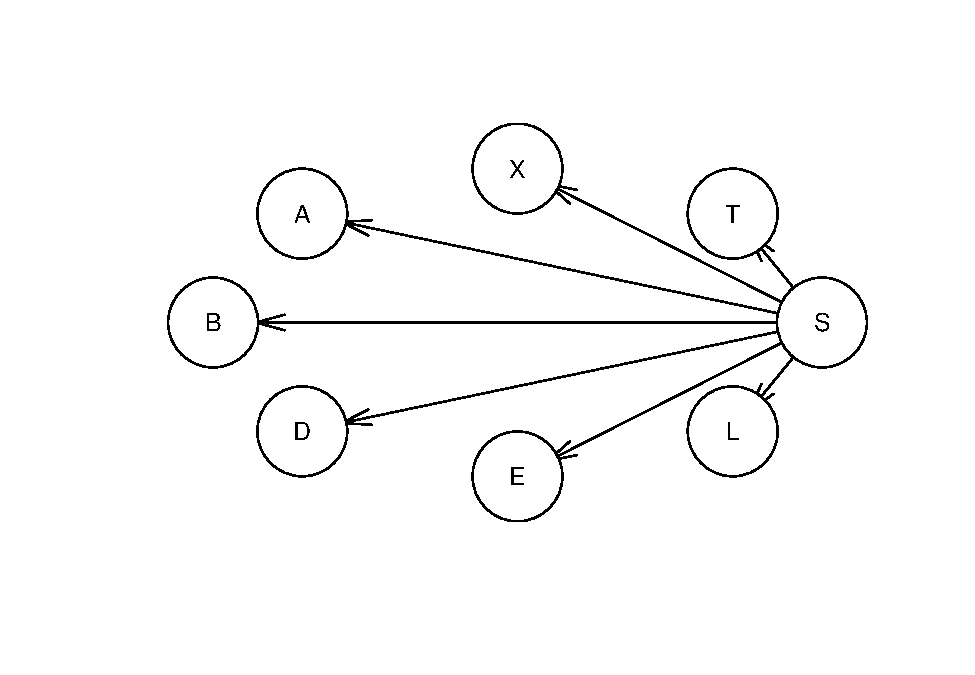
\includegraphics{Lab1_graphical_models_alive213_files/figure-latex/unnamed-chunk-6-1.pdf}

\begin{Shaded}
\begin{Highlighting}[]
\CommentTok{#compare results with given BN dag}
\NormalTok{BN_dag_parameters =}\StringTok{ }\KeywordTok{bn.fit}\NormalTok{(BN_dag, }\DataTypeTok{data =}\NormalTok{ train)}
\NormalTok{graphical_BN_dag =}\StringTok{ }\KeywordTok{as.grain}\NormalTok{(BN_dag_parameters)}
\NormalTok{BN_dag_tree =}\StringTok{ }\KeywordTok{compile}\NormalTok{(graphical_BN_dag)}

\NormalTok{conf_matrix_BN =}\StringTok{ }\KeywordTok{predict_BN}\NormalTok{(BN_dag_tree,nodes,pred_node, answer, observed) }
\CommentTok{#confusionmatrix for the NB network:}
\KeywordTok{print}\NormalTok{(conf_matrix_BN)}
\end{Highlighting}
\end{Shaded}

\begin{verbatim}
##       classify
## answer  no yes
##    no  359 154
##    yes 180 307
\end{verbatim}

\begin{Shaded}
\begin{Highlighting}[]
\CommentTok{#Misclassification rate for the NB network:}
\KeywordTok{missclass_rate}\NormalTok{(conf_matrix_BN)}
\end{Highlighting}
\end{Shaded}

\begin{verbatim}
## [1] 0.334
\end{verbatim}

We get an higher missclassification rate, and therefore less correct
predictions/result of S. This is because of the we have a different
markov blanket for S, and the assumption of independencies between the
other nodes in the network, when using the Bayesian classifier.
Trade-off is a simpler model with less computation, but a worsen result
in prediction.

\hypertarget{task-5---explain-why-you-obtain-the-same-or-different-results-in-the-exercises-2-4.}{%
\subsection{Task 5 - Explain why you obtain the same or different
results in the exercises
(2-4).}\label{task-5---explain-why-you-obtain-the-same-or-different-results-in-the-exercises-2-4.}}

In exercise 2-3 we obtain the same results, this is due to all networks
having the same Markov blanket, which are the nodes S depend on. In
Exercise 5 we have a different markov blanket, with a naive assumption
of independence between nodes in the network (except for S), which gives
us a higher misclassification rate (and less accurate predictions).

\end{document}
